\documentclass[mathserif]{beamer}
\usetheme{Boadilla}
%\usepackage[francais]{babel}
\usepackage[utf8]{inputenc} % Uses the utf8 input encoding
\usepackage[T1]{fontenc} % Use 8-bit encoding that has 256 glyphs
\usepackage[style=authoryear,backend=biber]{biblatex}
\addbibresource{main.bib}
\usepackage{etoolbox}
\makeatletter
\patchcmd{\@@description}{\advance\beamer@descdefault by
  \labelsep}{\advance\beamer@descdefault by -1em}{}{}
\makeatother

\usepackage{calc}
\usepackage{xcolor}

\AtBeginSection[]
{
\setbeamercolor{section in toc}{fg=alerted text.fg}
\setbeamercolor{section in toc shaded}{bg=structure!20,fg=structure}
\setbeamertemplate{section in toc shaded}[default][100]
\begin{frame}<beamer>
  \frametitle{Outline}
  \tableofcontents[currentsection,hideallsubsections]
\end{frame}
}

\definecolor{myorange}{RGB}{180,90,0}

\definecolor{mygreen}{RGB}{70,140,0}

\newcommand{\mycite}[1]{{\color{mygreen} \small #1}}

\usepackage[nomath]{kpfonts}
\usepackage{eulervm}
%\usepackage{default}

\usepackage{amsthm}
\usepackage{amssymb}
\usepackage{xparse}
\usepackage{thmtools}
\usepackage{stackrel}

%shortcuts
\newcommand{\R}{\mathbb{R}}
\newcommand{\C}{\mathbb{C}}
\newcommand{\Z}{\mathbb{Z}}
\newcommand{\N}{\mathbb{N}}
\newcommand{\fii}{\varphi}
\newcommand{\dd}{\mathrm{d}}
\newcommand{\CP}{\mathbb{CP}}
\renewcommand{\S}{\mathbb{S}}
\DeclareMathOperator{\Sp}{Sp}
\DeclareMathOperator{\tr}{tr}
\DeclareMathOperator{\dist}{dist}

% theorems configuration

\makeatletter
\newtheoremstyle{indented}
{7pt} %vertical space before
{7pt} % vertical space after
{} %{\addtolength{\@totalleftmargin}{2.5em}
	%\addtolength{\linewidth}{-3.5em}
	%\parshape 1 3.5em \linewidth} %body font
{1.5em} %indent
{\bfseries} %header font
{.} %punctuation
{.5em} %horizontal space after header
{} %header specification

\theoremstyle{definition}

\newtheorem{defn}{Définition}[section]

\theoremstyle{plain}
%\newtheorem*{theorem*}{Theorem}

\newtheorem{thm}{Théorème}

\renewcommand{\thetheorem}{\Alph{theorem}}
\newenvironment{preuve}{
	\noindent \textbf{Proof. }}{\hfill $\square$\medskip\par}

\newtheorem{exemple}[defn]{Example}
\newtheorem{prop}[defn]{Proposition}
\newtheorem{corr}[defn]{Corollary}
\newtheorem{por}[defn]{Porisme}
\newtheorem{ex}[defn]{Example}
\newtheorem{lem}[defn]{Lemma}
\newtheorem{conj}{Conjecture}
\newtheorem{ax}{Axiom}  %Axioms have their own numerotation

\theoremstyle{definition}
\newtheorem{rem}[defn]{Remark} %remarks are not indented
\newtheorem{rems}[defn]{Remarks}

%--------------
% Mise en page mathématique
%--------------
\addtolength{\jot}{.2em}


\title{Szeg\H{o} kernels and Toeplitz operators}
\author{Alix Deleporte}
\date{September 22, 2020}
\institute[LMO]{Laboratoire de Mathématiques d'Orsay\\Université Paris-Saclay}
\newcommand{\spline}{\hline}
\renewcommand{\arraystretch}{1.3}

\DeclareSourcemap{
  \maps[datatype=bibtex]{
    \map[overwrite=true]{
      \step[fieldsource=author,
            match=Deleporte,
            final]
      \step[fieldset=keywords, fieldvalue=Deleporte]
    }
  }
}
\begin{document}

\beamertemplatenavigationsymbolsempty

    \expandafter\def\expandafter\insertshorttitle\expandafter
       }%\insertframenumber}


\begin{frame}
	\titlepage
      \end{frame}

      \begin{frame}
  \frametitle{Positions}
  2016--2019: PhD (Strasbourg)

  \vfill

  2019: Postdoc (MSRI, Berkeley)

  \vfill

  2020: Postdoc (Zürich)
  
  \vfill
  
  2020--20??: Maître de Conférences (LMO, Paris-Saclay)
\end{frame}

      \begin{frame}
        \frametitle{Outline}
        \begin{enumerate}\setcounter{enumi}{-1}
        \item Motivation: antiferromagnetic spin systems
          \begin{itemize}
          \item What are spin systems?
          \item Frustration in antiferromagnets
          \end{itemize}
        \item Basics of Toeplitz quantization
          \begin{itemize}
          \item What is Toeplitz quantization?
          \item The case of the sphere: spin systems
          \item Semiclassical analysis
          \end{itemize}
        \item Localisation of low-energy states
          \begin{itemize}
          \item Localisation at first order
          \item Localisation at second order
          \item Applications to frustrated spin systems
          \end{itemize}
        \end{enumerate}
      \end{frame}

\begin{frame}
  \frametitle{Introduction}
  \begin{itemize}
  \item<1-> {\bfseries spin systems}: models for magnetism in solids.
  \item<2-> {\bfseries classical spins}: one atom at site $i$
    $\rightsquigarrow$ one spin $s_i\in \S^2$.
  \item<3> Heisenberg antiferromagnet: Graph $G=(V,E)$,
    
    search the minima of the following energy:
    \[
      (s_i)_{i\in V}\mapsto\sum_{i\sim j}s_i\cdot s_j.
    \]
    Here $i\sim j$ when the atoms $i$ and $j$ are neighbours in $G$
    and $\cdot$ is the scalar product.
  \end{itemize}
\end{frame}

             \begin{frame}
         \frametitle{Introduction}
   \begin{center}
     \begin{picture}(50,100)
           \only<1>{\put(-125,-80){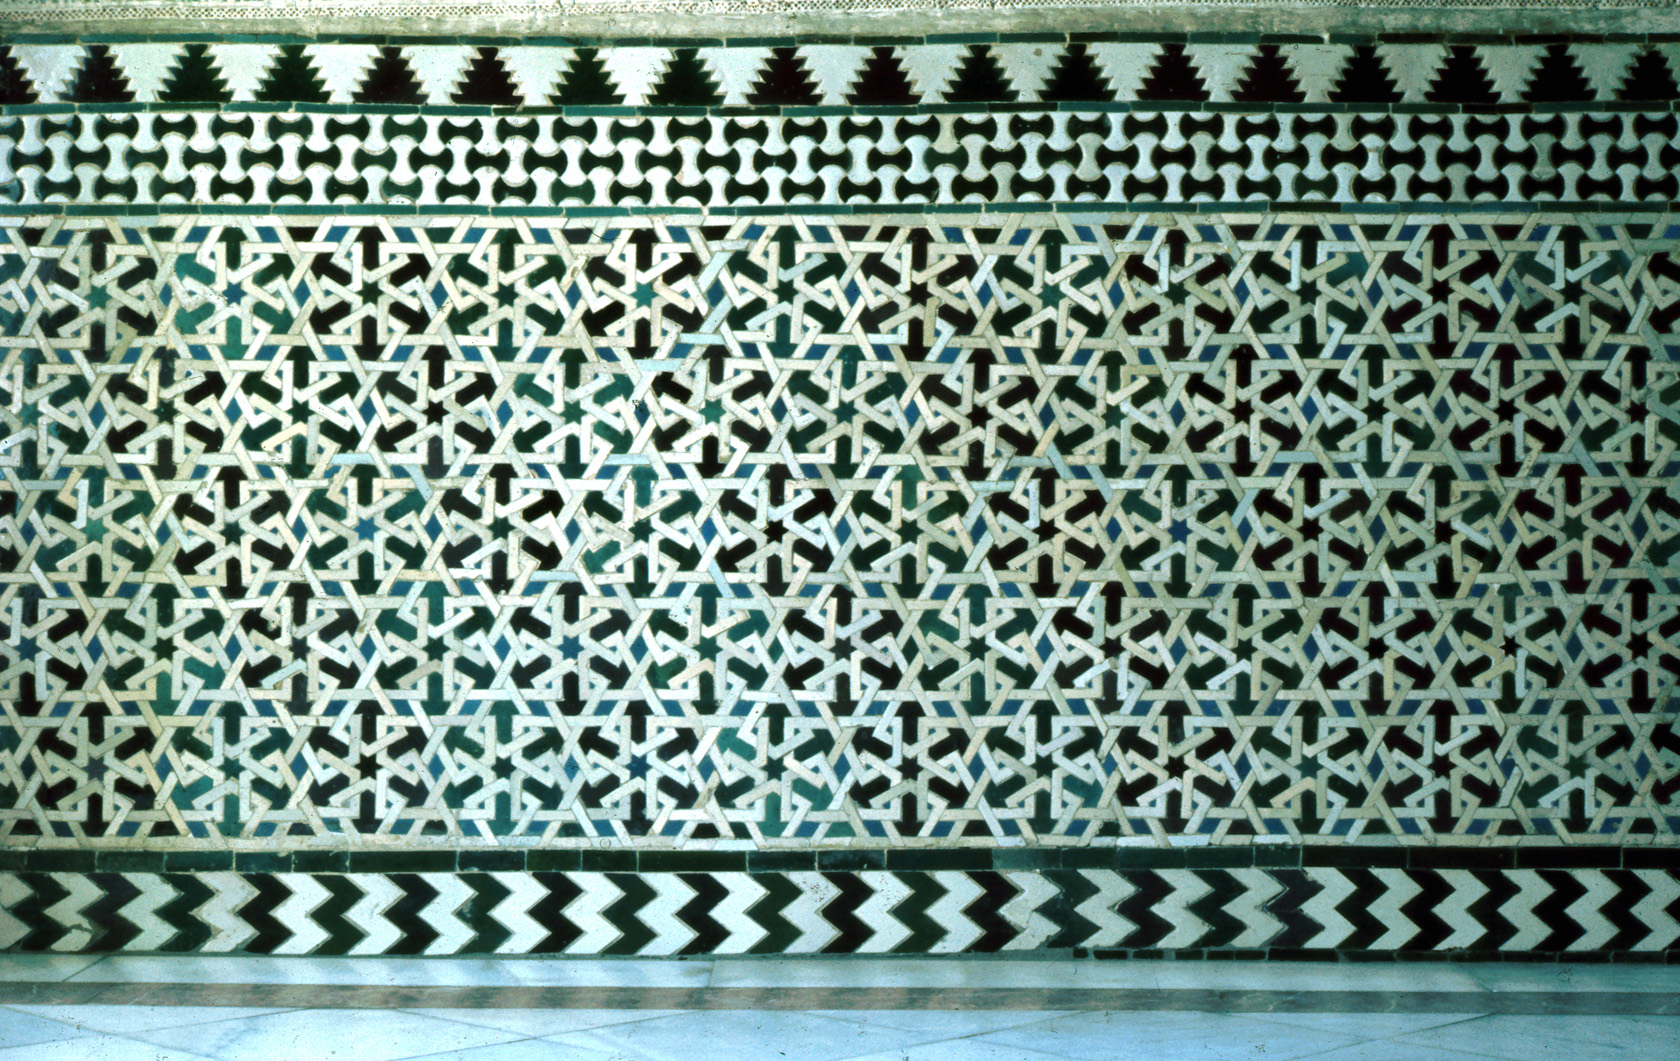
\includegraphics[scale=9]{Alcazar.png}}}
           \only<2>{\put(-125,-80){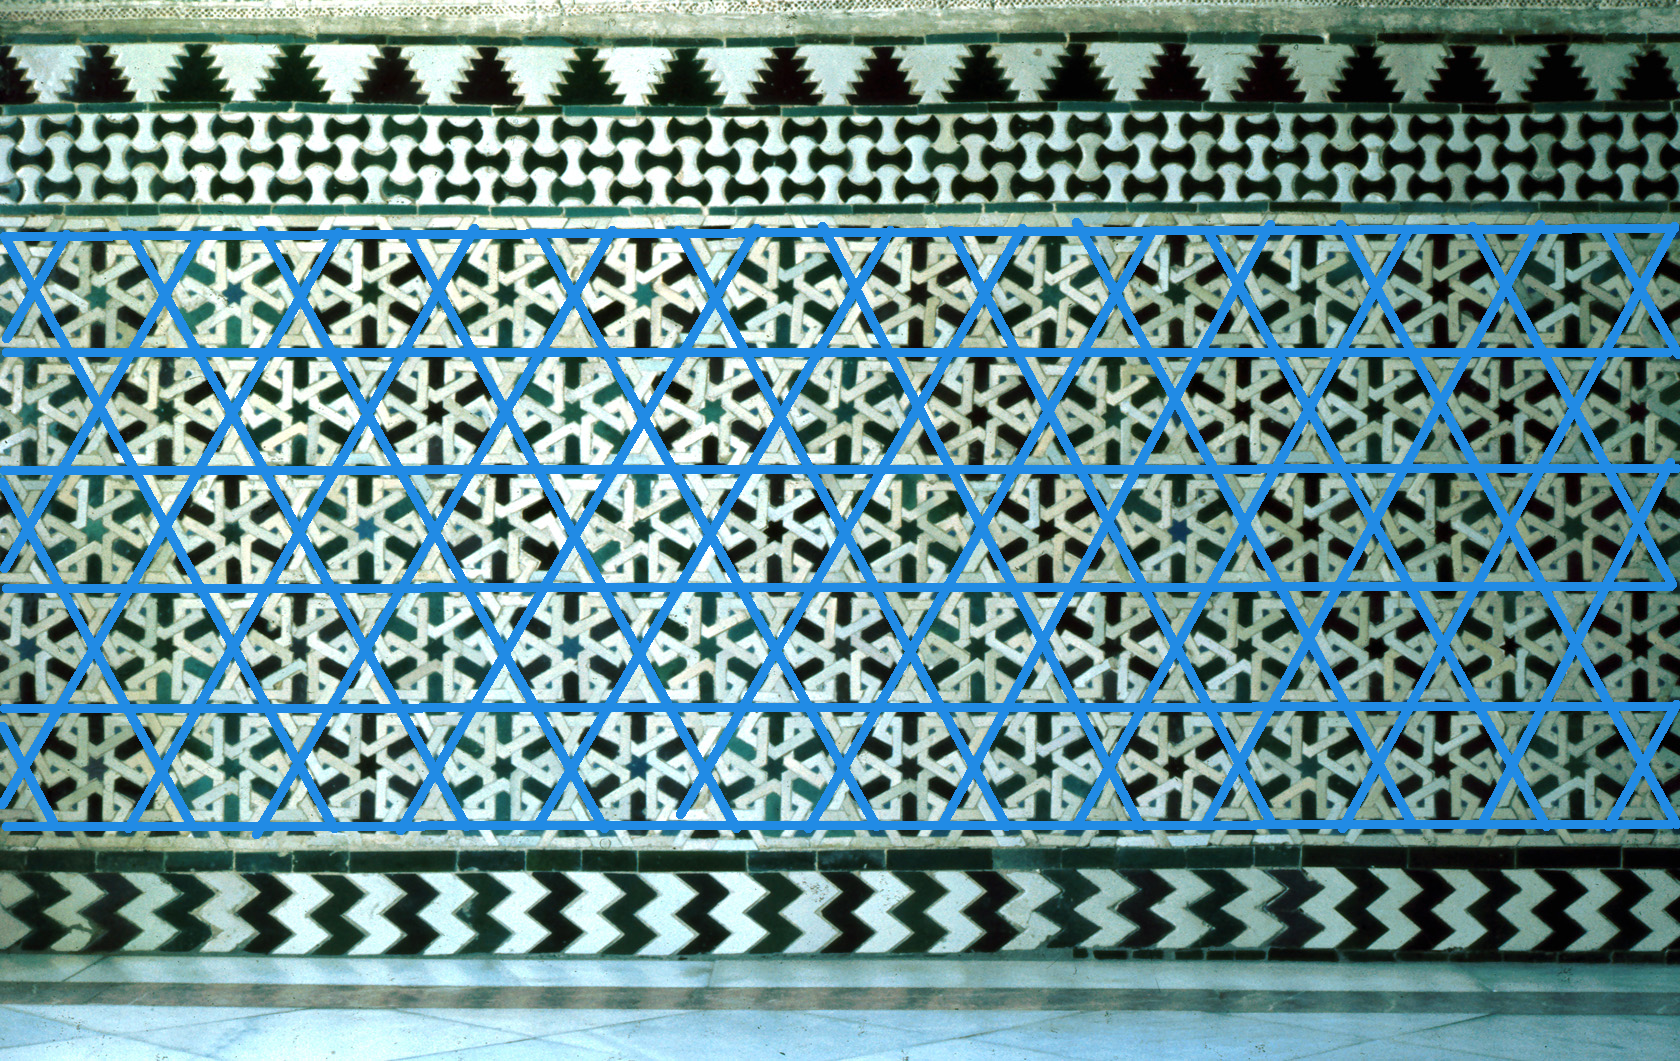
\includegraphics[scale=9]{Alcazar-Kagome.png}}}
           \only<3>{\put(-112,-80){\includegraphics[scale=0.32]{kagome-svg.png}}}
           \only<4>{\put(-112,-80){\includegraphics[scale=0.32]{kagome-spins-svg.png}}}
           \only<5>{\put(-112,-80){\includegraphics[scale=0.32]{kagome-spins-2-svg.png}}}
         \end{picture}
         \vspace{8em}

         Kagome lattice: \uncover<2->{appears in Zn$_2$CU$_3$(OH)$_6$Cl$_2$ crystals.}
       \end{center}
     \end{frame}

     \begin{frame}\frametitle{Introduction}
       \begin{itemize}
       \item Quantum spin: self-adjoint matrices
         $S_x,S_y,S_z\in M_{N+1}(\C)$ \[[S_x,S_y]=\frac{2i}{N}S_z\qquad
           [S_y,S_z]=\frac{2i}{N}S_x\qquad [S_z,S_x]=\frac{2i}{N}S_y.\]
       \item Several spins $\rightarrow$ {\color{myorange} tensor product}.
         \[S_{x,i}=\underbrace{Id\otimes \cdots\otimes Id}_{i-1}\otimes S_x\otimes
           \underbrace{Id\otimes
             \cdots
             \otimes
             Id}_{d-i}.\]
         
       \item<2>
         Quantum
         energy
         (matrix
         of
         size
         $(N+1)^d$):
         \[
           \sum_{i\sim j}S_{i,x}S_{j,x}+S_{i,y}S_{j,y}+S_{i,z}S_{j,z}.\]
         
         
      \end{itemize}
    \end{frame}
    \begin{frame}
      \frametitle{Introduction}
      Quantum energy is a self-adjoint matrix $\Rightarrow$
      
      \hspace{1em}eigenvalues
      $\lambda_1\leq \lambda_2\leq \cdots\leq \lambda_{(N+1)^d}$

      \hspace{1em}and associated eigenvectors. \vspace{1em}
      
      Goal: {\color{myorange} qualitative study of eigenvectors} associated with
      $\lambda_1$ (ground states) or other small eigenvalues.
      
      \hfill
      
      \uncover<2>{Physics claim: {\color{myorange} quantum-classical
          correspondence} as $N\to +\infty$.
        
        \hfill
        
      Prediction \mycite{[Douçot-Simon 1998]}: lowest-energy eigenvectors concentrate on {\color{myorange} some} classical configurations.}
    \end{frame}
      \begin{frame}
        \frametitle{Introduction}
        Toeplitz quantization:
        \begin{itemize}
          \item treat $N\to +\infty$ as a semiclassical
       limit
     \item see eigenvectors above as sections over $(\S^2)^d$.
     \end{itemize}
     \uncover<2->{Questions:}
     \begin{itemize}
        \item<2-> Where does the ground state concentrate?
        \item<3> What is the decay speed outside the concentration set?
        \end{itemize}
      \end{frame}

      \begin{frame}
        \frametitle{Introduction}
        \setbeamercovered{transparent}
        {\footnotesize
        \begin{description}
        \item<1>[{[D. 2019]}] Alix Deleporte. “Low-Energy Spectrum of Toeplitz Operators: The Case
of Wells.” In: Journal of Spectral Theory 9 (2019).
\item<1-2> [{[D. 2020a]}] Alix Deleporte. “Low-Energy Spectrum of Toeplitz Operators with a
Miniwell.” In: Comm. Math. Phys 378(3), 1587-1647.
\item<1>[{[D. 2018a++]}] Alix Deleporte. “Quantum Selection for Spin Systems.” In: arXiv
1808.00718 (2018).
\item<1>[{[D. 2018b++]}] Alix Deleporte. “The Bergman Kernel in Constant Curvature.” In:
arXiv 1812.06648 (2018).
\item<1-2>[{[D. 2020b]}] Alix Deleporte. “Toeplitz Operators with Analytic Symbols.” In: Journal of Geometric Analysis, to appear.
\item<1>[{[D. 2019++]}] Alix Deleporte. “WKB Eigenmode Construction for Analytic Toeplitz
  Operators.” In: arXiv 1901.07215 (2019).
  \item<1-2>[{[D. 2020c]}] Alix Deleporte. ``Fractional exponential
    decay in the forbidden region for Toeplitz operators.'' In: Documenta Mathematica (to appear)
  
        \end{description}}
      \end{frame}

      

\section{Basics of Toeplitz quantization}
\begin{frame}
  \frametitle{Quantization: I}
\begin{center}
	\begin{tabular}{|c|c|}
		\spline
	    Classical mechanics & Quantum mechanics\\
		\spline
		\uncover<2->{Symplectic manifold $M$} & \uncover<2->{Hilbert Space $H$}\\ 
		\spline 
		\uncover<3->{Function $p\in C^{\infty}(M,\R)$}& \uncover<3->{Self-adjoint
                                                   operator $P\in L(H)$}\\
		\spline
          \uncover<4->{Hamiltonien flow $\Phi_t(p)$} &
                                                  \uncover<4->{Unitary
                                                        flow $e^{itP/\hbar}$}\\
		\spline
		\uncover<5->{Poisson Bracket} &\uncover<5->{Lie Bracket}\\
		\spline
	\end{tabular}\end{center}\vspace{0em}
	\uncover<6>{Quantization : associate to $p\in
          C^{\infty}(M,\R)$ a family $Op_{\hbar}(p)\in L(H)$, such that, as
          $\hbar \to 0$,
          \[
            [Op_{\hbar}(p),Op_{\hbar}(q)]=i\hbar Op_{\hbar}(\{p,q\})+O(\hbar^2).
          \]
          
          \vfill
          
          Semiclassical analysis: study $Op_{\hbar}(p)$ as $\hbar\to 0$.}
          
          
      \end{frame}

\begin{frame}
  \frametitle{Quantization: II}
  Quantization: associate {\bf classical dynamics} (driven by
  real-valued functions) with {\bf self-adjoint operators}.

Ingredients: a symplectic manifold $(M,\omega)$, a Lagrangian
distribution $\mathcal{F}\subset TM$.

\vfill

{\bfseries Step 1}: construct the {\bfseries prequantum bundle} $L$
over $M$: it is a $\C$-bundle with Hermitian structure, and curvature
$2i\pi \omega$.

{\bfseries Step 2}: associate to $f:M\to \R$ an operator $Op(f)$
acting on $\mathcal{F}$-invariant sections of $L$.
\end{frame}

\begin{frame}
  \frametitle{Quantization: III}
  {\bfseries Semiclassical limit}: replace $\omega$ with $N\omega$ for
  $N\in \N$ large (replace $L$ with $L^{\otimes N}$).

  \vfill

  Example 1:
  \begin{itemize}
  \item 
  $M=T^*X$, $X$ Riemannian manifold,
  $\mathcal{F}=\mathrm{span}(\partial/\partial \xi)$.
\item 
  $\mathcal{F}$-invariant sections of
  $L^{\otimes N}$ are functions on $X$.
\item $Op$ is
  Weyl-quantization. ($\xi\rightsquigarrow iN^{-1}\partial_x$).
\end{itemize}

\vfill

Example 2:
\begin{itemize}
\item $M$ is a Kähler manifold (compatible complex structure $J$),
  $\mathcal{F}=\mathrm{span}(\partial/\partial \overline{z})$.
\item $\mathcal{F}$-invariant sections of $L^{\otimes N}$ are
  holomorphic sections.
\item $Op$ is Toeplitz-quantization.
\end{itemize}
\end{frame}


\begin{frame}
  \frametitle{Toeplitz quantization}
  \begin{itemize}
  \item Quantum space $H_N(M)$ of holomorphic sections of
  $L^{\otimes N}$.
\uncover<2->{\item Szeg\H{o} projector $S_N:L^2(M,L^{\otimes N})\to H_N(M).$}
  \end{itemize}
  \uncover<3->{The Szeg\H{o} projector has an integral kernel (section
    over $M^2$):
    \[
      (S_Nu)(x)=\int_M S_N(x,y)u(y) \omega^{\wedge d}(dy).
    \]
  }

  \vfill
  
  \uncover<4->{ Let $f\in L^{\infty}(M,\C)$. The Toeplitz operator associated
  with $f$ is the bounded operator
\begin{center}
\begin{array}{rcl}
 		T_N(f):H_N(M)&\to & H_N(M)\\
		u& \mapsto& \uncover<5>{S_N(}fu\uncover<5>{)}.
 		\end{array}
\end{center}}
\end{frame}

\subsection{Case of the sphere}

\begin{frame}
  \frametitle{Case $M=\S^2$}
  Stereographic chart: $L$ is topologically trivial.

  \hspace{9.5em}Its hermitian metric is
  $\frac{1}{1+|z|^2}|\cdot|^2.$ \[H_N(M)\simeq \left\{f\text{ holo on $
        \C$},\,\int_{\C}\cfrac{|f|^2}{(1+|z|^2)^{N+2}}<\infty\right\}=\C_N[X].\]
 \uncover<2->{Expression of the Szeg\H{o}
 kernel in this chart:\[S_N(z,w)=\cfrac{N+1}{\pi}\left(\cfrac{1+z\overline{w}}{\sqrt{(1+|z|^2)(1+|w|^2)}}\right)^N.\]}
\uncover<3->{
  \only<1-3>{\[T_N(\text{base coords})=\vphantom{\frac{N-2}{N}}\text{spin matrices}.\]}
  \only<4>{\[T_N(\S^2\ni (x,y,z)\mapsto x)=\frac{N-2}{N}S_x.\]}
  }
\end{frame}

\subsection{Semiclassical limit}
\begin{frame}
  \frametitle{The Szeg\H{o} kernel}
 On $\S^2$, there holds $S_N(x,y)=\frac{(N+1)}{\pi}\Psi^{\otimes
      N}(x,y)$, where $\Psi$ is a fixed section over $M\times M$ and
    $|\Psi|\approx e^{-c\dist(x,y)^2}$.
    \uncover<2->{\begin{theorem}[\mycite{[Delin 1998]}]
        Let $M$ be a compact, $C^2$ Kähler manifold of
        dimension $d$. Then
        \[
          |S_N(x,y)|<CN^d\exp(-c\sqrt{N}\dist(x,y)).
        \]
      \end{theorem}
    }
    \uncover<3->{\begin{theorem}[\mycite{[Charles 2003]}]
        Suppose $M$ is $C^{\infty}$. There exists a section
        $\Psi$ and a sequence of functions $(s_k)_{k\geq 0}$ on
        $M\times M$ such that
      \[
        S_N(x,y)=N^d\Psi^{\otimes
          N}(x,y)(s_0+N^{-1}s_1+\cdots)(x,y)+O(N^{-\infty}).
      \]
      Here, for some $c>0$,
      \[
        |\Psi(x,y)|\leq e^{-c\dist(x,y)^2}.
        \]
      \end{theorem}}
    
\end{frame}


\begin{frame}
  \frametitle{Approaches for Szeg\H{o} kernel estimates}
  Off-diagonal decay:
  \begin{itemize}
  \item Spectral gap for $\overline{\partial}^*\overline{\partial}$
    \mycite{[Kohn 1963, Hörmander 1968]}.
  \item Off-diagonal $\exp(-c\sqrt{N})$ decay \mycite{[Christ 1991,
      Delin 1998]}.
  \item Off-diagonal $\exp(-cN)$ decay if $M$ is {\color{myorange} real-analytic}
    \mycite{[Berndtsson-Berman-Sjöstrand 2008]}.
  \end{itemize}

  Near diagonal estimates:
  \begin{itemize}
    \item FIOs with complex phase \mycite{[Shiffman-Zelditch 2002,
        Charles 2003]}: versions of
      the result above, remainder $O(N^{-\infty})$, following
      \mycite{[Boutet de Monvel-Sjöstrand 1975]}.
    \item Weighted estimates on $-\Delta$
      \mycite{[Ma-Marinescu 2007, Ma-Marinsecu-Kordyukov 2019]}:
      generalisations.
    \item Analytic calculus \mycite{[\underline{D. 2018c++},
        Rouby-Vũ Ng\d{o}c-Sjöstrand 2018++]}: if $M$ is
      {\color{myorange} real-analytic},
      the remainder is $O(e^{-cN})$ with $c>0$.
    \end{itemize}
  \end{frame}

  \begin{frame}
    \frametitle{Application: Kodaira embeddings}
    Let $M$ be a compact Kähler manifold with a prequantum bundle $L$.

    For $N$ large, with $\mathop{dim}(H^0(M,L^{\otimes N}))=d_N$, and
    $(s_k)$ an orthonormal basis, let
    \begin{center}
      \begin{array}{rcl}
        \phi_N:M&\to &\C\mathbb{P}^{d_N-1}\\
        x&\mapsto &[s_1(x):s_2(x):\cdots:s_{d_N}(x)]
      \end{array}
    \end{center}
    Then $\phi_N$ is a well-defined complex map (because
    $S_N(x,x)=\sum |s_k(x)|^2$, they don't all vanish at the same
    point).
    \vfill
    \uncover<2>{
      \begin{itemize}
      \item $\Phi_N$ is an embedding for $N$ large. \mycite{[Kodaira 1954]}
      \item The pulled-back Fubini metric is close (up to scaling) to
        the original metric. \mycite{[Tian 1990, Zelditch 2000]}
      \end{itemize}
      }
  \end{frame}

  \begin{frame}
    \frametitle{Application: Calculus of Toeplitz operators}

    \begin{theorem}[{\mycite{[Schlichenmaier 1999]}}]Let $M$ be smooth. Let $a$ and $b$ be
      smooth real-valued functions on $M$. Then there exists a sequence $(c_k)_{k\geq
        0}\in (C^{\infty}(M,\R))^{\N}$ such that
      \[
        T_N(a)T_N(b)=T_N(c_0+N^{-1}c_1+\cdots)+O(N^{-\infty}).
        \]

        If $a$ does not vanish, then there exists a sequence
        $(d_k)_{k\geq 0}\in (C^{\infty}(M,\R))^{\N}$ such that
        \[
          T_N(a)T_N(d_0+N^{-1}d_1+\cdots)=S_N+O(N^{-\infty}).
          \]
        \end{theorem}
        Calculus in analytic regularity (up to $O(e^{-cN})$):
        \mycite{[\underline{D. 2018c++}]}.
  \end{frame}


\section{Localisation of low-energy states}

\subsection{Localisation at the classical minimal set}
\begin{frame}
  \frametitle{Speed of localisation}
 For $N\in \N$, let $u_N$ be a normalised eigenvector associated with
 the smallest eigenvalue of $T_N(f)$. Let $Z=\mathop{argmin}(f)$.
  \begin{theorem}[\mycite{[Charles 2000]}]
  If f is {\color{myorange}smooth} and $U\subset M$ is at positive distance from $Z$, then \[\int_{U}|u_N|^2=O(N^{-\infty}).\]\vspace{-1.2em}
\end{theorem}
\uncover<2>{
\begin{theorem}[\mycite{[\underline{D. 2018c++}]}]
If f is {\color{myorange}real-analytic} then\vspace{-1em}
      \[
        \int_{U}|u_N|^2=O(e^{-cN}).%\vspace{-0.5em}
      \]
    \end{theorem}}
  Tool: calculus of Toeplitz operators.
\end{frame}
\begin{frame}
  \frametitle{Speed of localisation -- improved}
  \begin{theorem}[\mycite{[\underline{D. 2020++}]}]
    If $f$ is {\color{myorange} smooth} and $U\subset M$ is at
    positive distance from $Z$, then
    \[
      \int_U |u_N|^2=O(e^{-cN^{\alpha}}).
      \]
    \end{theorem}
    \uncover<2>{
      \begin{itemize}
        \item $M$ is $C^{1,1}$: $\alpha=\frac 14$.
        \item $M$ is analytic: $\alpha=\frac 13$.
        \item $f$ is Lipschitz: $\alpha=\frac 12$, one can take
          $U=\{f\geq \min(f)+CN^{-\frac 12+\epsilon}\}$.
        \item $f$ is $C^2$: $\alpha=\frac 12$, one can take $U=\{f\geq
          \min(f)+CN^{-1+\epsilon}\}$.
        \end{itemize}
      }
      
      \vfill

      Tool: off-diagonal decay of the projector.
    \end{frame}


\subsection{Subprincipal effects on localisation}

\begin{frame}
  \frametitle{Characteristic value}
  \begin{itemize}
  \item For $x\in Z$ a minimal point for $f$, we construct $\mu(x)$
    associated with the Hessian of $f$ at $x$.
  \item $\mu$ captures the eigenvalue contribution of order $N^{-1}$.
  \item<2-> {\color{myorange} Quantum selection}: the ground states of $T_N(f)$
    concentrate only on the subset $Z_{\mu}$ of $Z$ where also $\mu$ is minimal.
  \end{itemize}
  
  \uncover<3>{\begin{itemize}
    \item case of a Schrödinger operator $-\hbar^2\Delta+V$
      \mycite{[Helffer-Sjöstrand 1986]}, where
      \begin{itemize}
      \item $V$ vanishes on a smooth submanifold $Z$
      \item Its transverse Hessian is nondegenerate on $Z$.
      \end{itemize}
    \item case of a magnetic Schrödinger operator with similar
    conditions \mycite{[Helffer-Morame 1996, Helffer-Kordyukov 2009]} .
    \end{itemize}
    }

\end{frame}

\begin{frame}
  \frametitle{Subprincipal localisation}
  Quantum selection in general for Toeplitz operators:
  \begin{theorem}[\mycite{[\underline{D. 2020?}]}]
    Let $M$ be smooth, let $f\in C^{\infty}(M,\R)$ and let $Z_{\mu}$ and
    $(u_N)_{N\geq 1}$ be as above.

    For all $U\subset M$ at positive distance from $Z_{\mu}$, one has
    \[
      \int_U
      |u_N|^2=O(N^{-\infty}).
      \]
  \end{theorem}
\end{frame}

\begin{frame}
  \frametitle{Particular case: frustrated spin systems}
  \begin{center}
    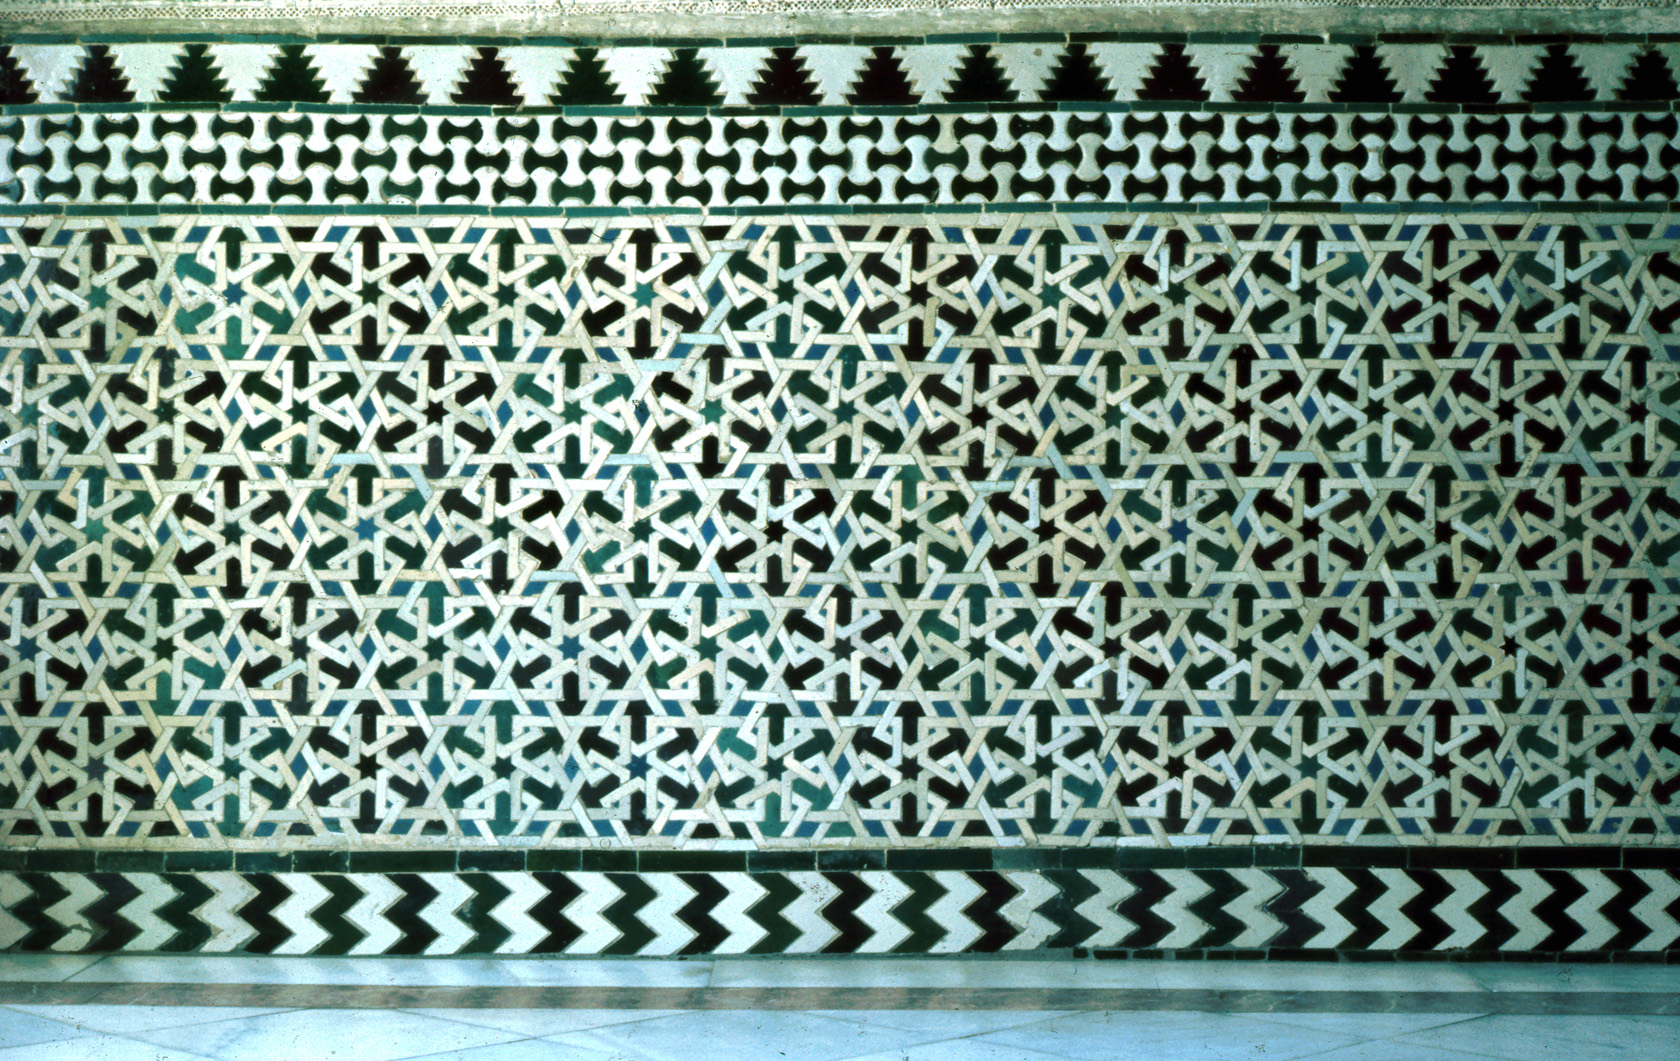
\includegraphics[scale=6]{Alcazar.png}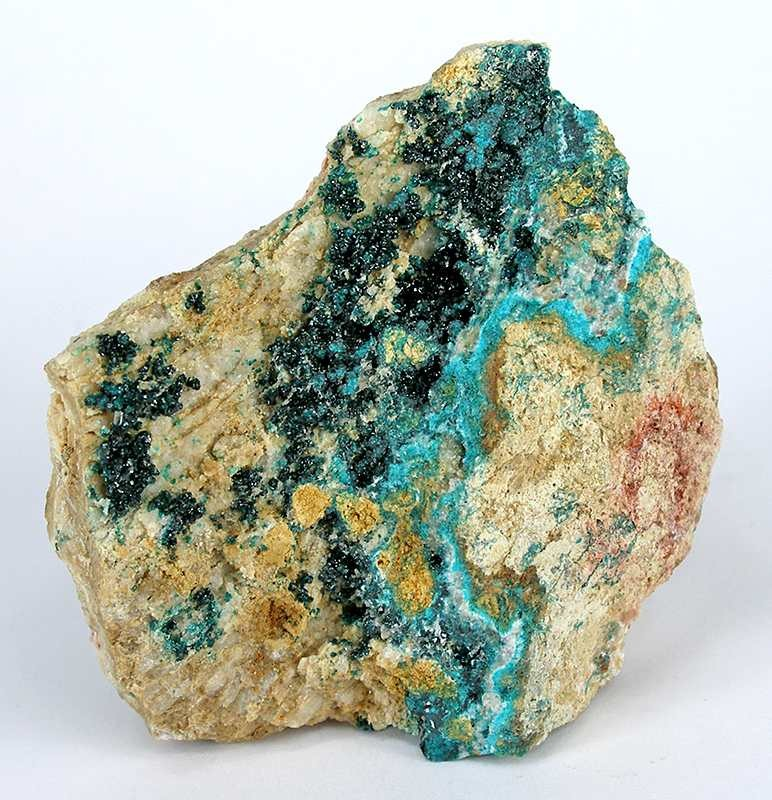
\includegraphics[scale=0.16]{Herbertsmithite.jpg}
  \end{center}
  \begin{itemize}
\item  Framework: fixed number of particles $d$, spin parameter $N$
  tends to infinity, set $Z$ arbitrarily complicated.

  \item<2->{Computations for this particular case
    $M=(\S^2)^d$ \mycite{[\underline{D. 2018b++}]}.}

  \item<3>{{\color{myorange} Open problem}: where is $\mu$ minimal among classical
      configurations on the Kagome lattice?}
  \end{itemize}
\end{frame}

\begin{frame}
  \frametitle{Applications: Mabuchi geodesics}
  Another application of localisation of eigenfunctions. (In progress,
  joint with S. Zelditch and P. Zhou)

  \vfill
  
  \begin{itemize}
  \item Riemannian structure (Mabuchi) on the space of Kähler metrics
  on $M$.
\item Geodesic equation $\Leftrightarrow$ complex Monge-Ampère
  equation.
\item<2-> {\color{myorange} Quantization} of the geodesics:
  (presumably) of the form $t\mapsto e^{tNT_N(f)}$.
\item<2-> Control of the spectrum of $T_N(f)$ allows us to study these operators.
  \end{itemize}
\end{frame}

\subsection{Future work}
\begin{frame}
  \frametitle{Perspectives}
    \begin{itemize}
    \item Second-order effects for a large number of spins.
    \item Low-energy dynamics.
    \item Non self-adjoint operators with analytic symbols (Scottish flag).
    \end{itemize}
  \end{frame}

  \begin{frame}
    \frametitle{Thanks}
    \centering 
    {\Large Thanks for your attention!}
  \end{frame}
  

  \begin{frame}[allowframebreaks]
    \frametitle{Bibliography}
        {\footnotesize
          \begin{description}
            \item[{[BS75]}] Louis Boutet de Monvel and Johannes
              Sjöstrand.  “Sur la singularité des noyaux de Bergman et
              de Szegö.” In: Journées équations aux dérivées
              partielles 34-35 (1975), pp. 123--164.
        \item[{[Cha00]}] Laurent Charles. “Aspects Semi-Classiques de La Quantification Géométrique.” PhD thesis. Université Paris 9, 2000.
        \item[{[Cha03]}] Laurent Charles. “Berezin-Toeplitz Operators, a Semi-Classical Approach.” en. In: Communications in Mathematical Physics 239.1-2
(Aug. 2003), pp. 1–28.
        \item[{[DS98]}] Benoît Douçot and Patrice Simon. “A Semiclassical Analysis of Order
from Disorder.” en. In: Journal of Physics A: Mathematical and General
31.28 (1998), p. 5855.
\item[{[HK09]}] Bernard Helffer and Yuri A. Kordyukov. “Semiclassical Analysis of
Schrödinger Operators with Magnetic Wells.” In: Contemporary Mathematics 500 (2009), p. 105.
\item[{[HM96]}] Bernard Helffer and Abderemane Mohamed. “Semiclassical Analysis for
the Ground State Energy of a Schrödinger Operator with Magnetic
Wells.” In: Journal of Functional Analysis 138.1 (1996), pp. 40–81.
\item[{[HS86]}] Bernard Helffer and Johannes Sjöstrand. “Puits Multiples En Limite
Semi-Classique V : Étude Des Minipuits.” In: Current topics in partial
differential equations (1986), pp. 133–186.
\item[{[HLX17++]}] Hamid Hezari, Zhiqin Lu, and Hang Xu. “Off-Diagonal Asymptotic
Properties of Bergman Kernels Associated to Analytic Kähler Potentials.” In: arXiv 1705.09281 (2017).
\item[{[Kor17++]}] Yuri A. Kordyukov. “On Asymptotic Expansions of Generalized Bergman
Kernels on Symplectic Manifolds.” In: arXiv 1703.04107 [math-ph]
(Mar. 2017).
\item[{[MM07]}] Xiaonan Ma and George Marinescu. Holomorphic Morse Inequalities
and Bergman Kernels. Vol. 254. Springer Science \& Business Media,
2007.
\item[{[RSV18++]}] Ophélie Rouby, Johannes Sjöstrand, and San Vũ Ng\d{o}c. “Analytic
Bergman Operators in the Semiclassical Limit.” In: hal-01851770 (July
2018).
\item[{[SZ02]}] Bernard Shiffman and Steve Zelditch. “Asymptotics of Almost Holomorphic Sections on Symplectic Manifolds.” In: J. reine angew. Math.
544 (2002), pp. 181–222.
        \end{description}
        }
      \end{frame}

\end{document}
%%% Local Variables:
%%% mode: latex
%%% TeX-master: t
%%% End:
